\chapter{Influence of Parks to Mitigate the Floods}

By now,  the best time to do the preparation to mitigate the severity of floods in Jakarta has been answered. The predictive modeling algorithm to estimate the number of districts as well as civilians that might be affected by floods with given rate of rainfall also have been built. Just now, the authorities are also already know which districts that they should focus their attention to during the heavy rainfall rate periods in Jakarta.\\

\noindent
The only thing that still missing is the question: how should people mitigate the floods? What should they do to mitigate the floods? It is a very tricky question to answer because of the need to use hefty amount of datasets with different variety of topics to find the solution.\\
 
\noindent
Unfortunately, there is no open dataset that might be helpful to answer this question. Also, the scope will be even broader if socioeconomics or sociological situation like the growing rate of populations or people's behavior on how they maintain the cleanliness of their environments are considered. The correlation between socieconomics or sociological situation with the occurrence of floods will be out of the scope of this project.\\

\noindent
Thus, to try to answer this question, a rather simplistic approach will be conducted. With Foursquare API, the parks nearby each district will be fetched. Then, the possible correlation between the amount of parks and the severity of floods will be investigated.\\

\noindent
In order to make sure that only venues with parks category will be returned, it is necessary to define the category ID of parks in advance before calling the API. Detailed information about different ID categories depending on the type of venues can be found in the Foursquare Developers page. Table \ref{tab:4} shows the output after Foursquare API was called.\\

\begin{table}
\centering
\caption{First five rows of places with parks category that were returned by Foursquare API}
\label{tab:4}
\begin{adjustbox}{width=\textwidth}
\begin{tabular}{llrrlrr}
\toprule
{} & District &  Latitude &   Longitude &                        Venue &  Venue Latitude &  Venue Longitude \\
\midrule
0 &     Koja &  -6.12075 &  106.907362 &            Taman Walang Baru &       -6.120104 &       106.905190 \\
1 &     Koja &  -6.12075 &  106.907362 &  JL. Lagoa Terusan gg. II C2 &       -6.110252 &       106.910098 \\
2 &     Koja &  -6.12075 &  106.907362 &                 Tanjungpriok &       -6.113818 &       106.893159 \\
3 &     Koja &  -6.12075 &  106.907362 &              Mochie's castle &       -6.131510 &       106.921496 \\
4 &     Koja &  -6.12075 &  106.907362 &  Food Park Mall Of Indonesia &       -6.118548 &       106.900294 \\
\bottomrule
\end{tabular}
\end{adjustbox}
\end{table}

\noindent
The first data that were returned from Foursquare API didn't look very good although the desired category of the place have already been defined in advance. The data contains not only parks, but also some other non-relevant places like restaurant and other places.  In order to fix this and to make sure that at the end the real parks is obtained, then the data needs to be filtered. All of the venues which doesn't contain the word 'taman', which is the Indonesian word for parks, will be excluded from the data. Table \ref{tab:5} shows the filtered data.\\

\begin{table}
\centering
\caption{Filtered table which only contains the real parks}
\label{tab:5}
\begin{adjustbox}{width=\textwidth}
\begin{tabular}{lrlrrlrr}
\toprule
{} &  index &   District &  Latitude &   Longitude &                Venue &  Venue Latitude &  Venue Longitude \\
\midrule
0 &      0 &       Koja & -6.120750 &  106.907362 &    Taman Walang Baru &       -6.120104 &       106.905190 \\
1 &      5 &   Cilandak & -6.289798 &  106.796926 &          Taman Gajah &       -6.277217 &       106.799566 \\
2 &     10 &   Cilandak & -6.289798 &  106.796926 &  Taman Tridarma Raya &       -6.303318 &       106.805154 \\
3 &     13 &  Kembangan & -6.191395 &  106.740586 &    Taman Meruya Ilir &       -6.195407 &       106.740664 \\
4 &     15 &  Kembangan & -6.191395 &  106.740586 &         Taman blok H &       -6.194011 &       106.737629 \\
\bottomrule
\end{tabular}
\end{adjustbox}
\end{table}

\noindent
From the filtered data, then the distribution of the amount of parks in Jakarta can be visualized using histogram. Figure \ref{fig=hist.png} shows the distribution of the amount of parks in Jakarta.\\


\begin{figure}
\begin{center}
\graphicspath{ {./Pict/} }
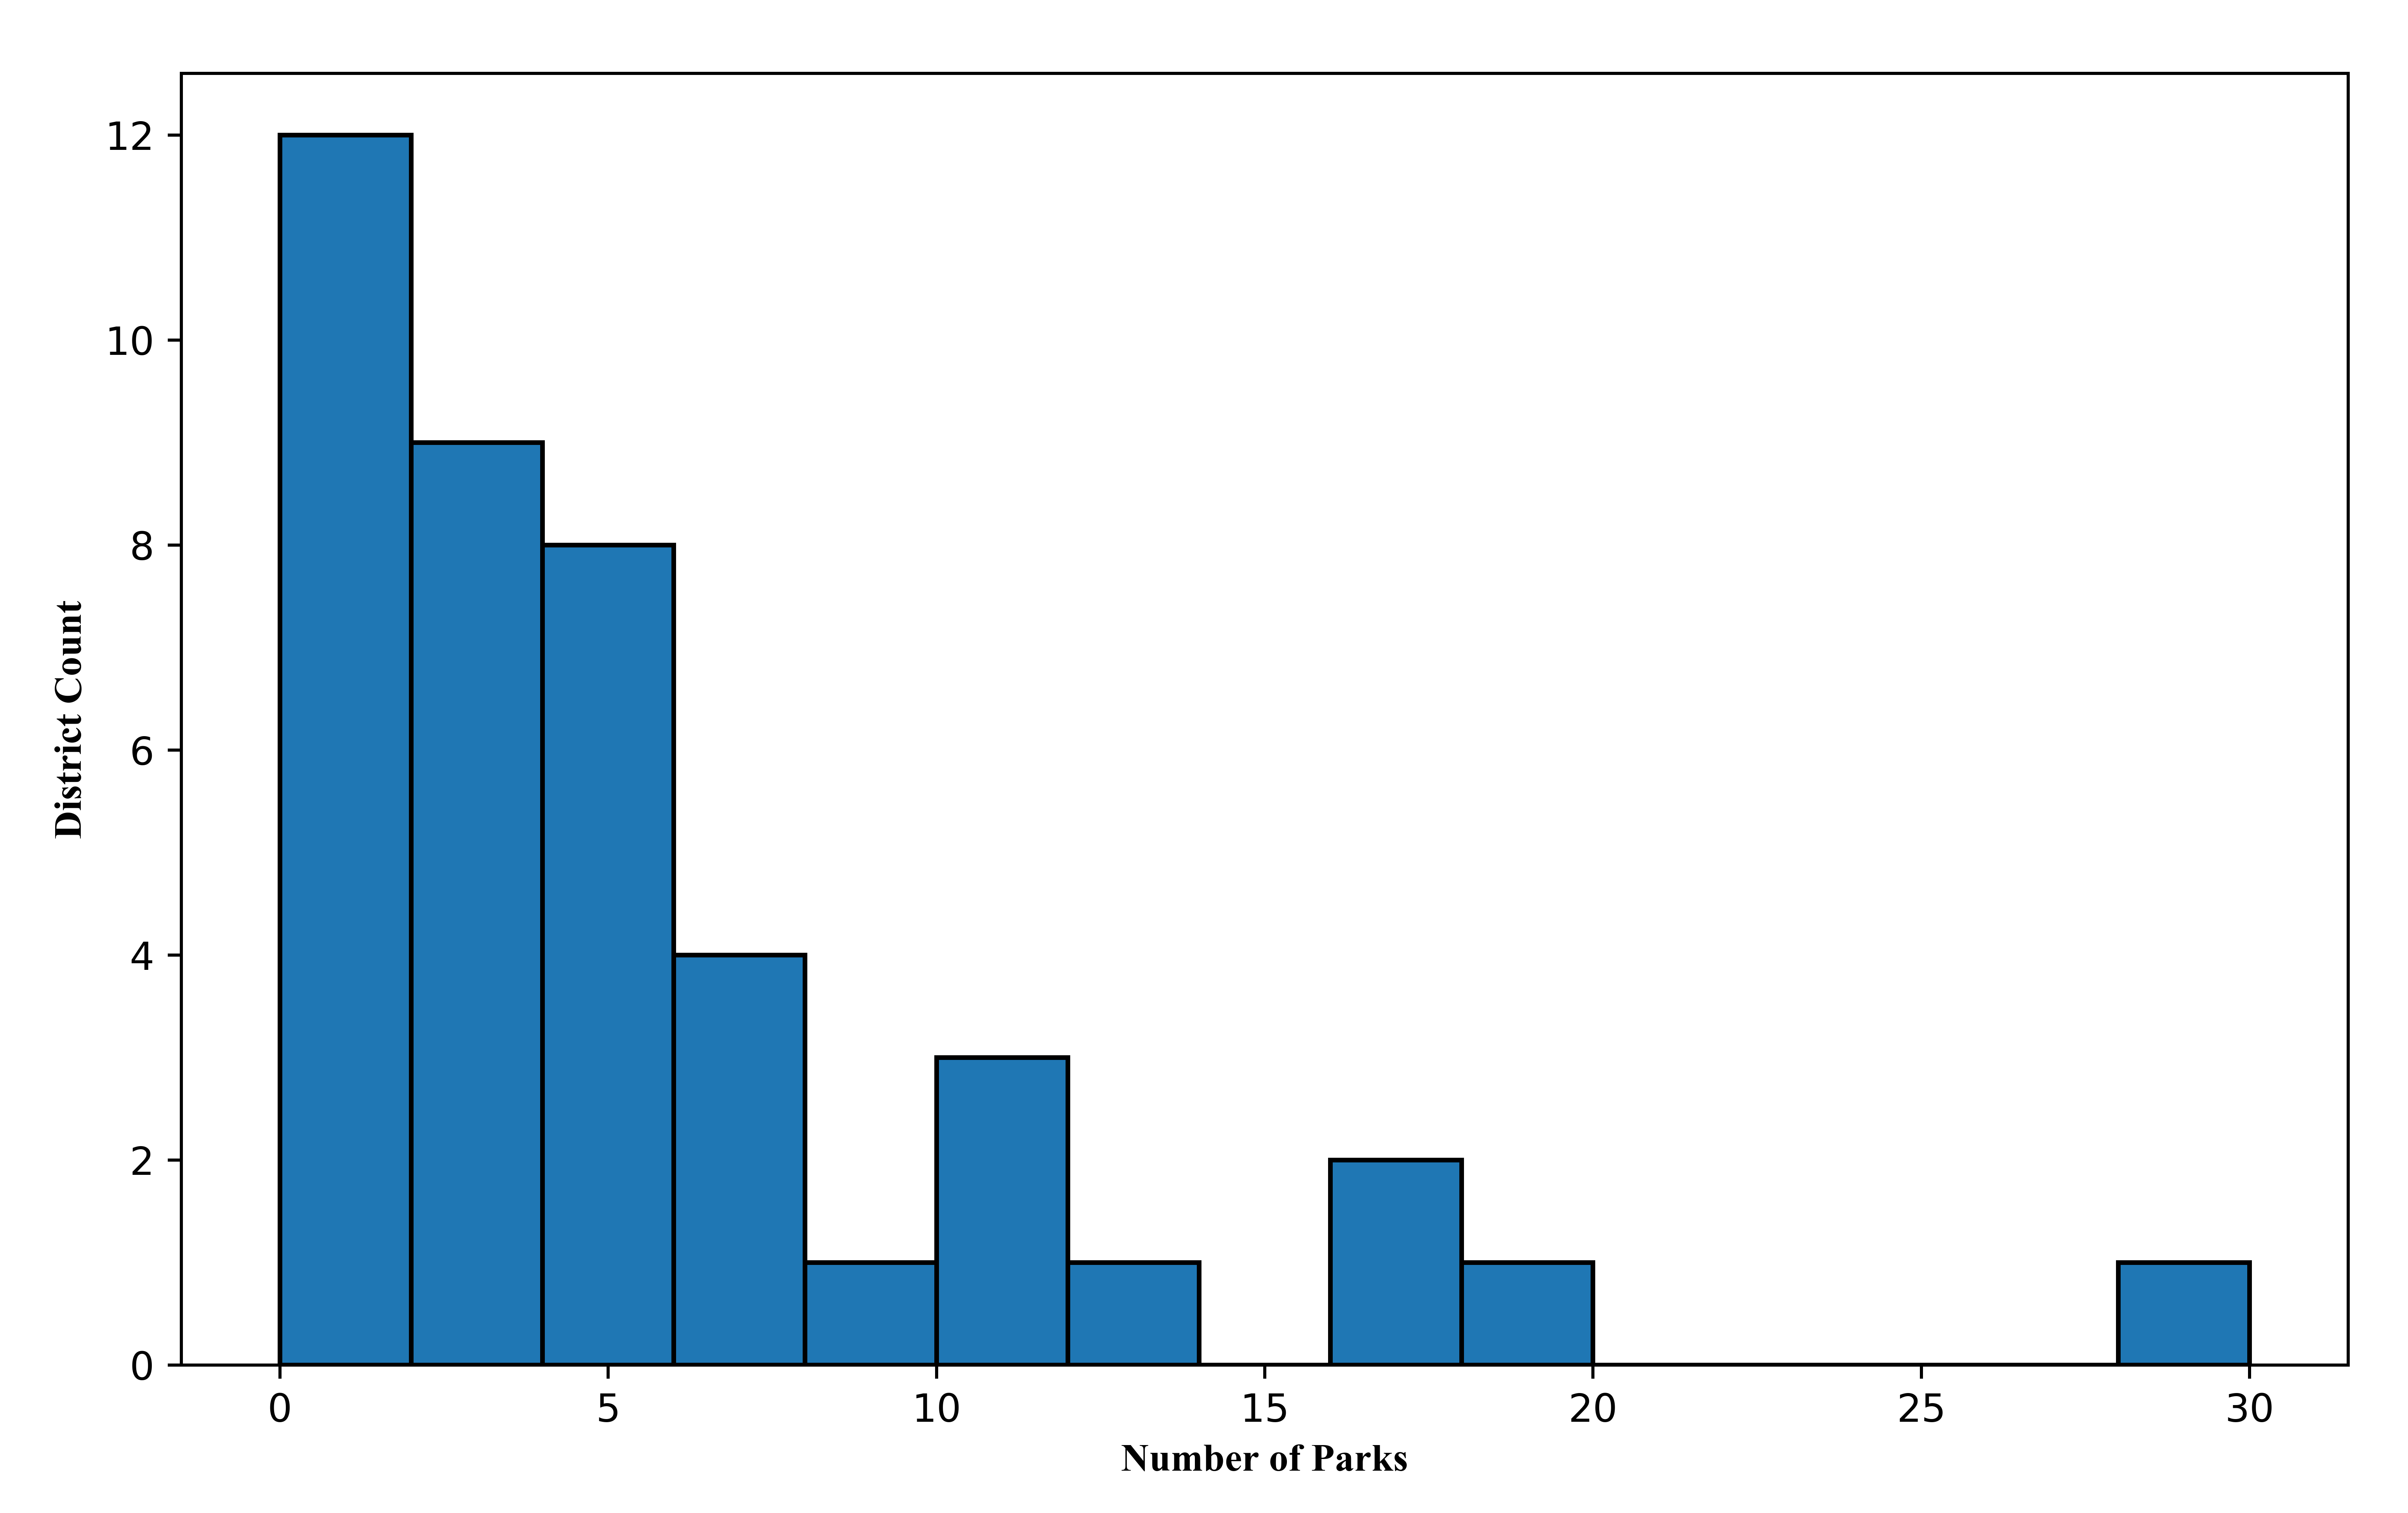
\includegraphics[scale=0.15]{hist.png}
\caption{Distributions of parks among Jakarta districts}\label{fig=hist.png}
\end{center}
\end{figure}

\noindent
As clearly seen from the histogram in Figure \ref{fig=hist.png}, the distribution of the amount of parks in Jakarta is heavily right-skewed. This means that the majority of the districts in Jakarta have a small number of parks. In fact, only 8 out of 41 districts have 10 or more parks. This is also one the problem in Jakarta that it is so congested with residential building and skyscrapers that there are not too many green spaces in the city.\\ 

\noindent
Having the data regarding the amount of parks in each district and then joined this data with the original data frame, then the correlation between them can be investigated. For this purpose, Pearson's correlation method is used. The Table \ref{tab:6} shows the Person's correlation results of all of the features in the data frame.\\

\begin{table}
\centering
\caption{Pearson's correlation result between features in the data frame}
\label{tab:6}
\begin{adjustbox}{width=\textwidth}
\begin{tabular}{lrrrrr}
\toprule
{} &  no. of cases &  no. of People Affected &  no. of People Forced to Relocate &  Days of Flood Recovery &      Park \\
\midrule
no. of cases                     &      1.000000 &                0.574098 &                          0.622585 &                0.942140 & -0.246997 \\
no. of People Affected           &      0.574098 &                1.000000 &                          0.854797 &                0.693484 & -0.188454 \\
no. of People Forced to Relocate &      0.622585 &                0.854797 &                          1.000000 &                0.780099 & -0.255296 \\
Days of Flood Recovery           &      0.942140 &                0.693484 &                          0.780099 &                1.000000 & -0.281488 \\
Park                             &     -0.246997 &               -0.188454 &                         -0.255296 &               -0.281488 &  1.000000 \\
\bottomrule
\end{tabular}
\end{adjustbox}
\end{table}

\noindent
From Table \ref{tab:6}, it can be concluded that the amount of parks in each district doesn't have a significant association with the severity of the floods. The Pearson's correlations between the amount of parks with different set of features are all in around -0.2. However, this negative correlation does makes sense since the more a district has a park, then the less the severity of the floods would be. It is important to note that the causality relationship between the amount of parks and the severity of floods cannot be drawn because no random assignment is involved.\\

\noindent
Nonetheless, although the amount of parks doesn't have a significant correlation with the severity of floods, but it is enough to encourage the districts to open up more green spaces in their area. Finally, Figure \ref{fig=parks.png} shows the data points between the amount of parks and the days needed for the districts to recover from flood.\\

\begin{figure}
\begin{center}
\graphicspath{ {./Pict/} }
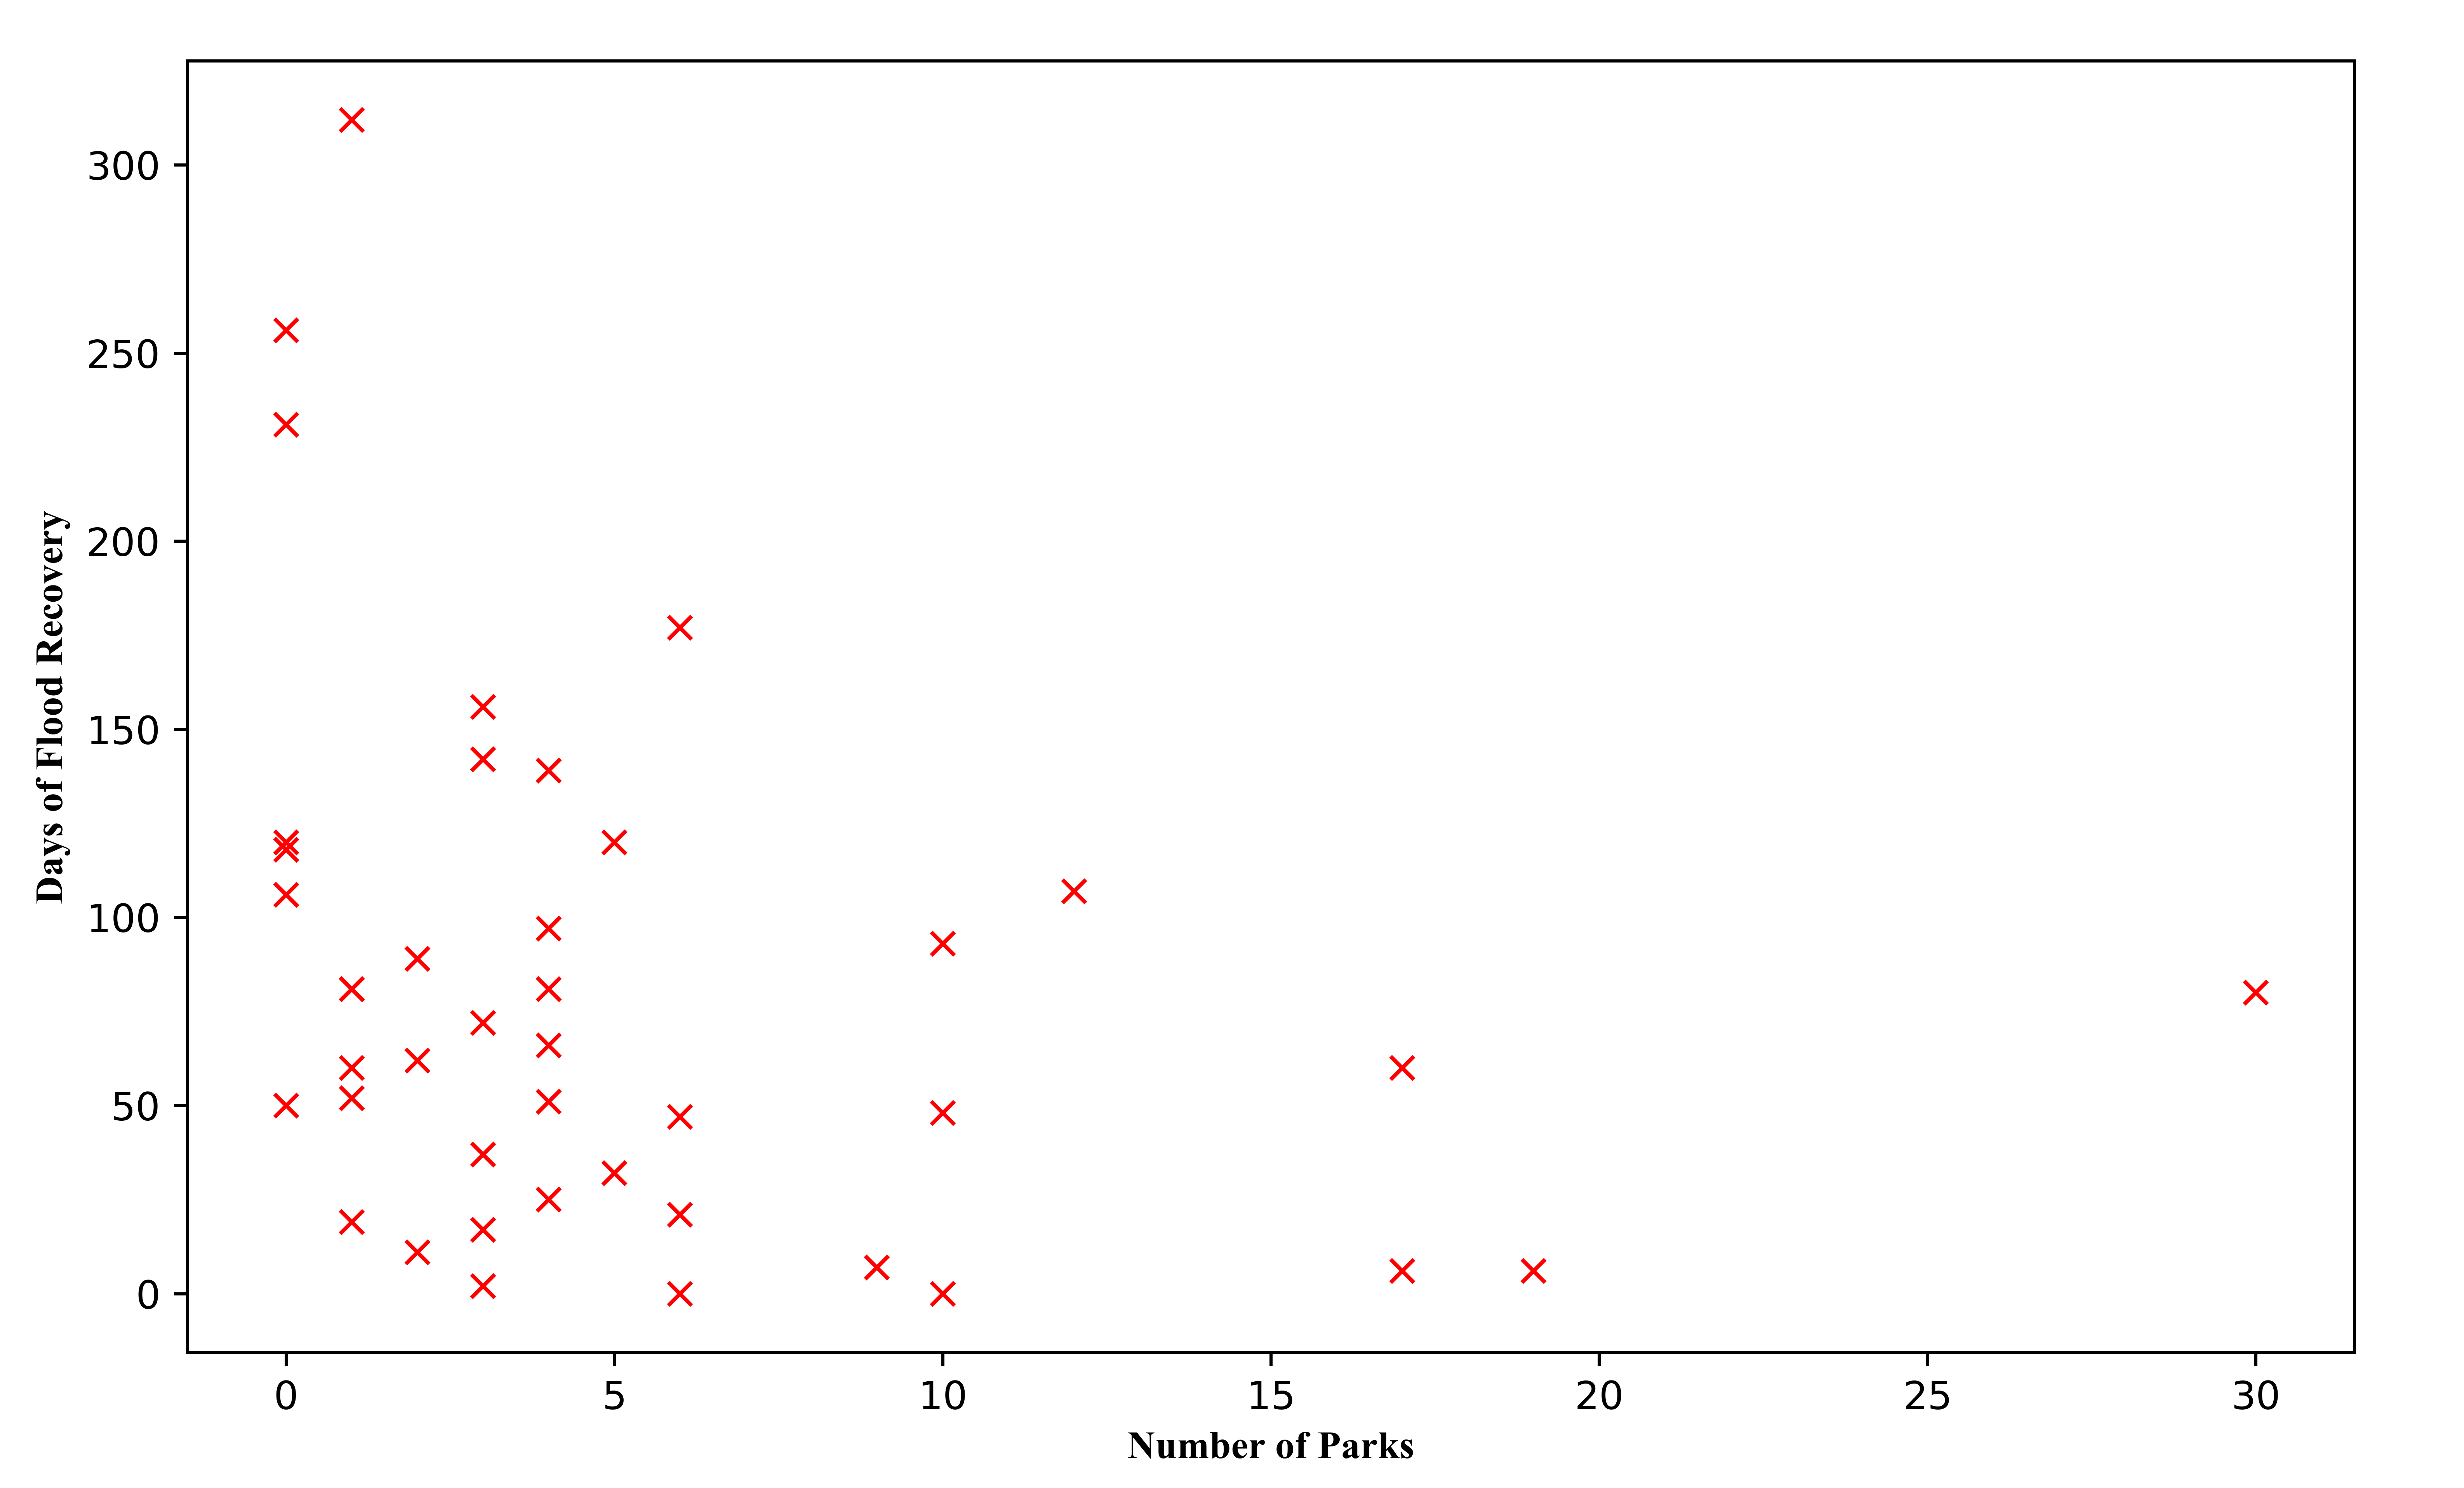
\includegraphics[scale=0.15]{parks.png}
\caption{Data points between the number of parks and the days needed for districts to recover from flood}\label{fig=parks.png}
\end{center}
\end{figure}
